% !TeX root = ../main.tex

\chapter{Solution Implementation}
\label{chap:solution-imp}

\section{Testing the LTC2945}
The LTC2945 testing was carried out using a Linear Tech eval board, DEMO CIRCUIT 1697A. Connections and modifications were made as follows:
\begin{itemize}
	\item VIN: tied to Arduino +5V
	\item GND: tied to Arduino GND
	\item ADIN: Tied to GND
	\item SCL: Tied to Arduino Pin D8 I2C2 SCL
	\item SDAI/SDAO (JP2 set to TIE): Arduino Pin D9 I2C2 SDA
	\item VPU: Tied to Arduino +3v3
	\item VOUT: Float or tied to dummy load (1k$\Omega$ to 10k$\Omega$)
	\item 20m$\Omega$ shunt replaced with 17$\Omega$ shunt for testing with $\sim$5k$\Omega$ load
	\item Installed 4.7k$\Omega$ pull up on I2C lines via R4, R5 footprints on EVB
\end{itemize}

\newpage
\subsection{Calculating Shunt Value for Test}
Using the 5V from the arduino as a source, and a load ranging 1k to 10k ohms, we calculate:
$$R_{L,min}=1k\Omega$$
$$V_{shunt}=V_S\frac{R_S}{R_L+R_S}$$
$$R_S=\frac{V_{Shunt}R_L}{V_s-V_{Shunt}}$$
$$V_{shunt}=0.1024V$$
$$R_{S,full scale}=\frac{(0.1024V)(1k\Omega)}{5V-0.1024V}=20.91\Omega$$
Adding some headroom, say, 15\%, and going to an E96 resistor value...
$$R_S=0.85(20.91)=17.8\Omega$$
Verifying for the high end of the range:
$$I_{min}=\frac{5V}{10k\Omega + 17.8\Omega}=499.1\mu A$$
$$V_{shunt, min}=(499.1\mu A)(17.8\Omega)=8.88mV$$
The shunt will range from 8.88mV to 87.44mV, within the ADC's usable range of 0V to 102.4mV.

\newpage
\subsection{Pictures of Evaluation Board, Display, and Phoebus Panels}
\begin{figure}[H]
	\centering
	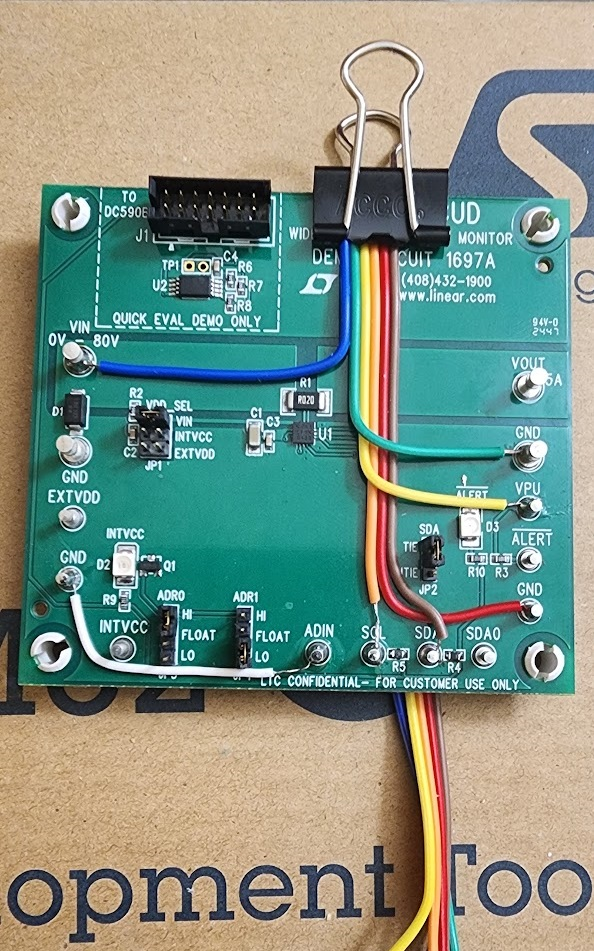
\includegraphics[
	width=3.5in,
	%height=0.85\textwidth,
	keepaspectratio
	]{Pictures/LTC2945_EVB_Original_Shunt}
	\caption{DEMO CIRCUIT 1697A Eval Board with Original Shunt, fly leads to connect to Arduino.}
\end{figure}

\begin{figure}[H]
	\centering
	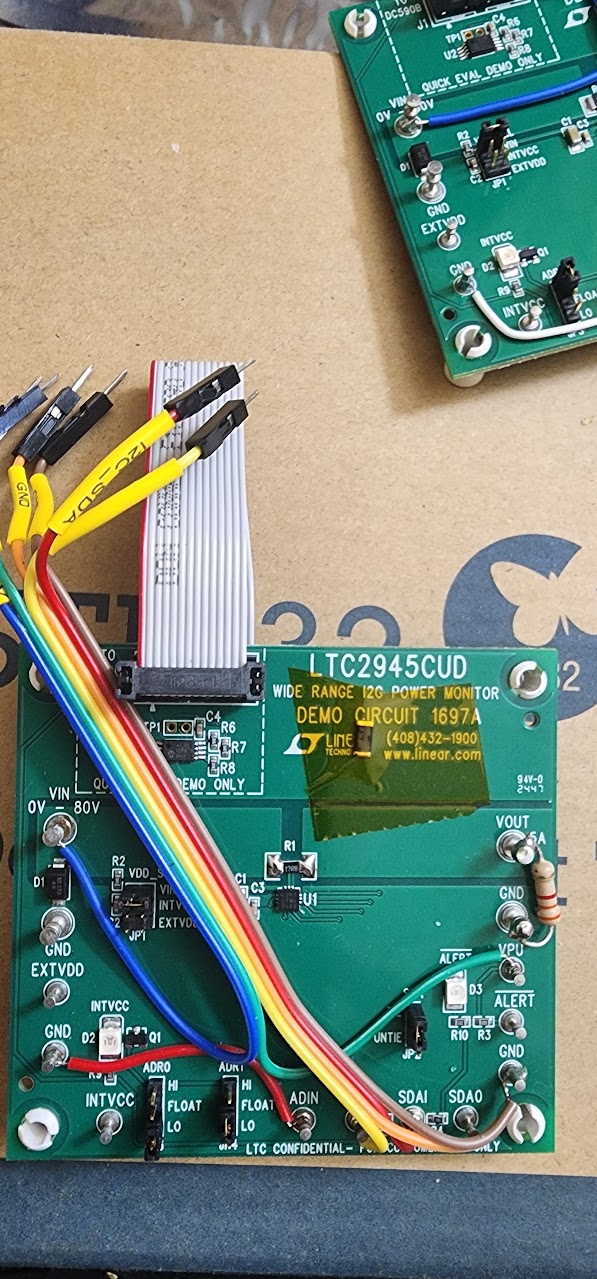
\includegraphics[
	width=3.5in,
	%height=0.85\textwidth,
	keepaspectratio
	]{Pictures/LTC2945_EVB_17Ohm_Shunt}
	\caption{DEMO CIRCUIT 1697A Eval Board with 17$\Omega$ Shunt, fly leads to connect to Arduino, and 4.7k$\Omega$ test load.}
\end{figure}

\begin{figure}[H]
	\centering
	\includegraphics[
	width=3.5in,
	%height=0.85\textwidth,
	keepaspectratio
	]{Pictures/ExampleDisplay-Single\_EVB_Connected\_Non-ALM}
	\caption{Arduino Giga with GIGA DISPLAY SHIELD showing dummy -5V rail being monitored, without alarm}
\end{figure}

\begin{figure}[H]
	\centering
	\includegraphics[
	width=3.5in,
	%height=0.85\textwidth,
	keepaspectratio
	]{Pictures/ExampleDisplay-Single\_EVB_Connected\_ALM}
	\caption{Arduino Giga with GIGA DISPLAY SHIELD showing dummy -5V rail being monitored, with UVL alarm, other channels I2C ALARM.}
\end{figure}

\begin{figure}[H]
	\centering
	\includegraphics[
	width=3.5in,
	%height=0.85\textwidth,
	keepaspectratio
	]{Pictures/ExampleDisplay-Single\_EVB\_Connected\_Non-ALM-3k3Load}
	\caption{Arduino Giga with GIGA DISPLAY SHIELD showing dummy -5V rail being monitored, without alarm, 3.3k$\Omega$ Load}
\end{figure}

\begin{figure}[H]
	\centering
	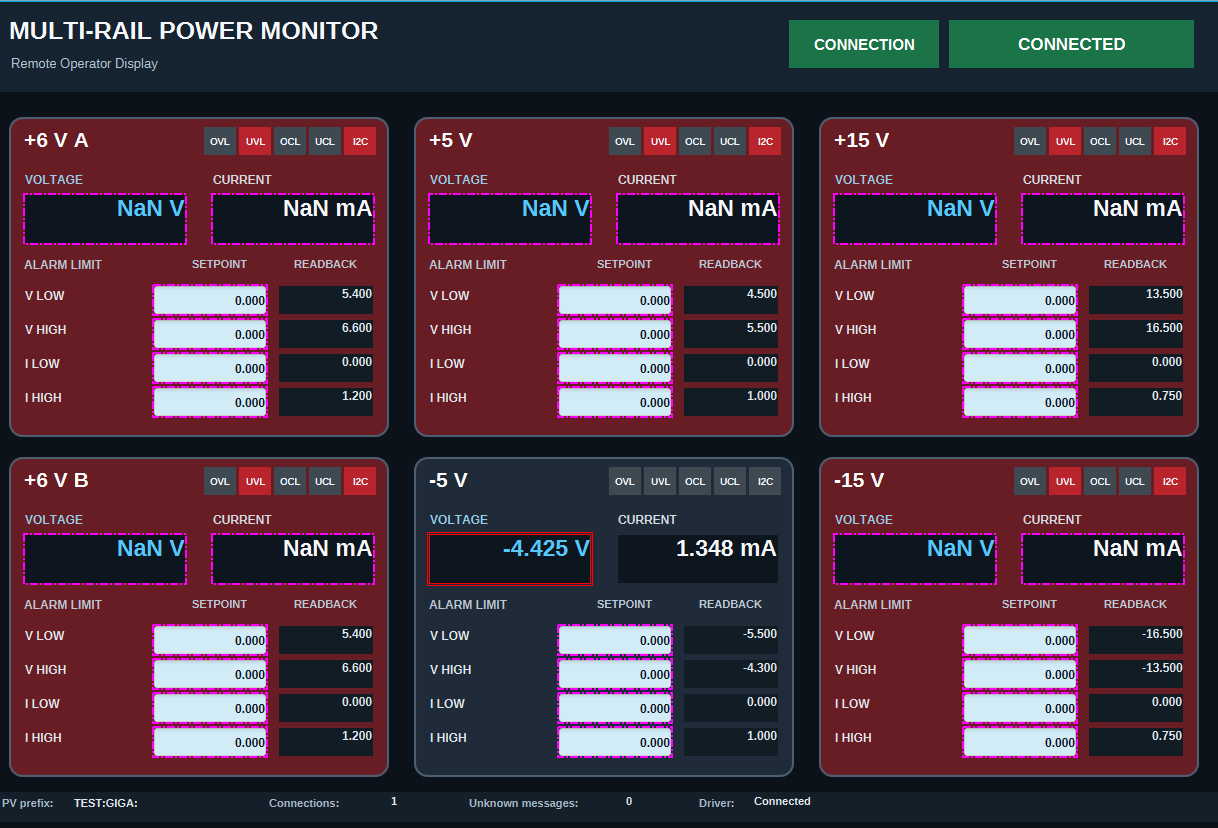
\includegraphics[
	width=\textwidth,
	%height=0.85\textwidth,
	keepaspectratio
	]{Pictures/Phoebus-SS-N5V-Test-3k3Load}
	\caption{Arduino Giga with GIGA DISPLAY SHIELD showing dummy -5V rail being monitored, without alarm, 3.3k$\Omega$ Load}
\end{figure}

\begin{figure}[H]
	\centering
	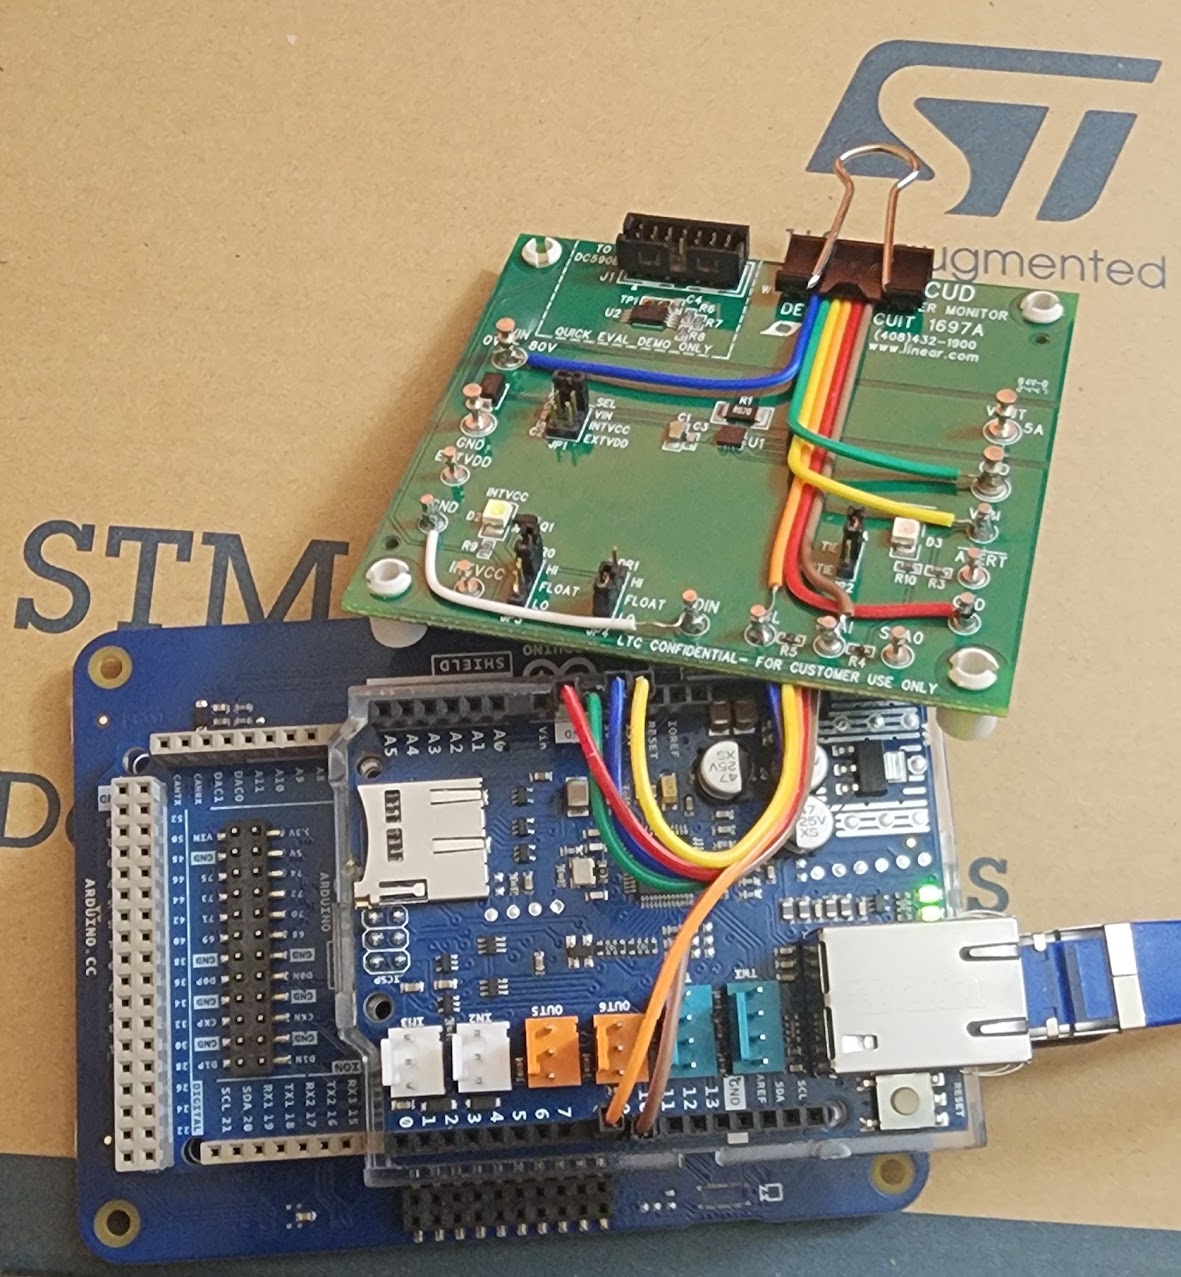
\includegraphics[
	width=\textwidth,
	%height=0.85\textwidth,
	keepaspectratio
	]{Pictures/EVBArduinoAssembly}
	\caption{Arduino Giga with GIGA DISPLAY SHIELD connected to an LTC2945 eval board}
\end{figure}

\section{Bring Up and Testing of the First Spin Board}
After construction of the printed circuit boards was complete, the board bring-up process was carried out prior to system-level testing.
The objective of the board bring-up process was to ensure that the electronic
operation of the circuitry was functioning, locate assembly problems and communication
issues, and make modifications if required before running the entire system.

In this case, initial testing was not done by powering up and trying to run the
entire system, but was carried out incrementally. Each rail, each signal and
functional block was tested separately so as to pinpoint failures without adding other
variables. Measurements were made with the use of a digital multimeter and
oscilloscope, whereas firmware and serial diagnostic output was used to ascertain if
the Arduino was communicating with peripheral devices.

Several problems were noted during this phase, but of primary concern was an error in
the I\textsuperscript{2}C Serial Data (SDA) interface between the circuitry of the
Arduino side and the isolated circuitry. This problem led to a failure of I\textsuperscript{2}C
communication and troubleshooting had to be done at the signal level with an
oscilloscope. The troubleshooting revealed that there was an incorrect selection of
a component in the constructed board, and temporary modification of the board was done
with the help of an additional logic inverter to fix the problem and allow further
development and testing of the system.

The subsequent sections describe the board bring-up process, detected failures,
measurements made for diagnostics, performed modifications, and the testing of the fixed
board.

\section{Assembly Verification/Visual Inspection and Smoke Test}
\subsection{Visual Inspection}
I hand-assembled all components of the boards, so a thorough visual inspection was carried out. The board was assembled using water-soluble paste flux and organic core water soluble 63/37 Sn/Pb solder wire (0.031" and 0.015"). As such, the boards were washed thoroughly prior to inspection.

Only one notable finding was found, U20 was shifted off the pads, with the exposed pad in the center having 'snapped' to pins 4/5/6. The board was reworked via hot air prior to power being applied to correct this. No other defects were found on visual inspection.

\begin{figure}[H]
	\centering
	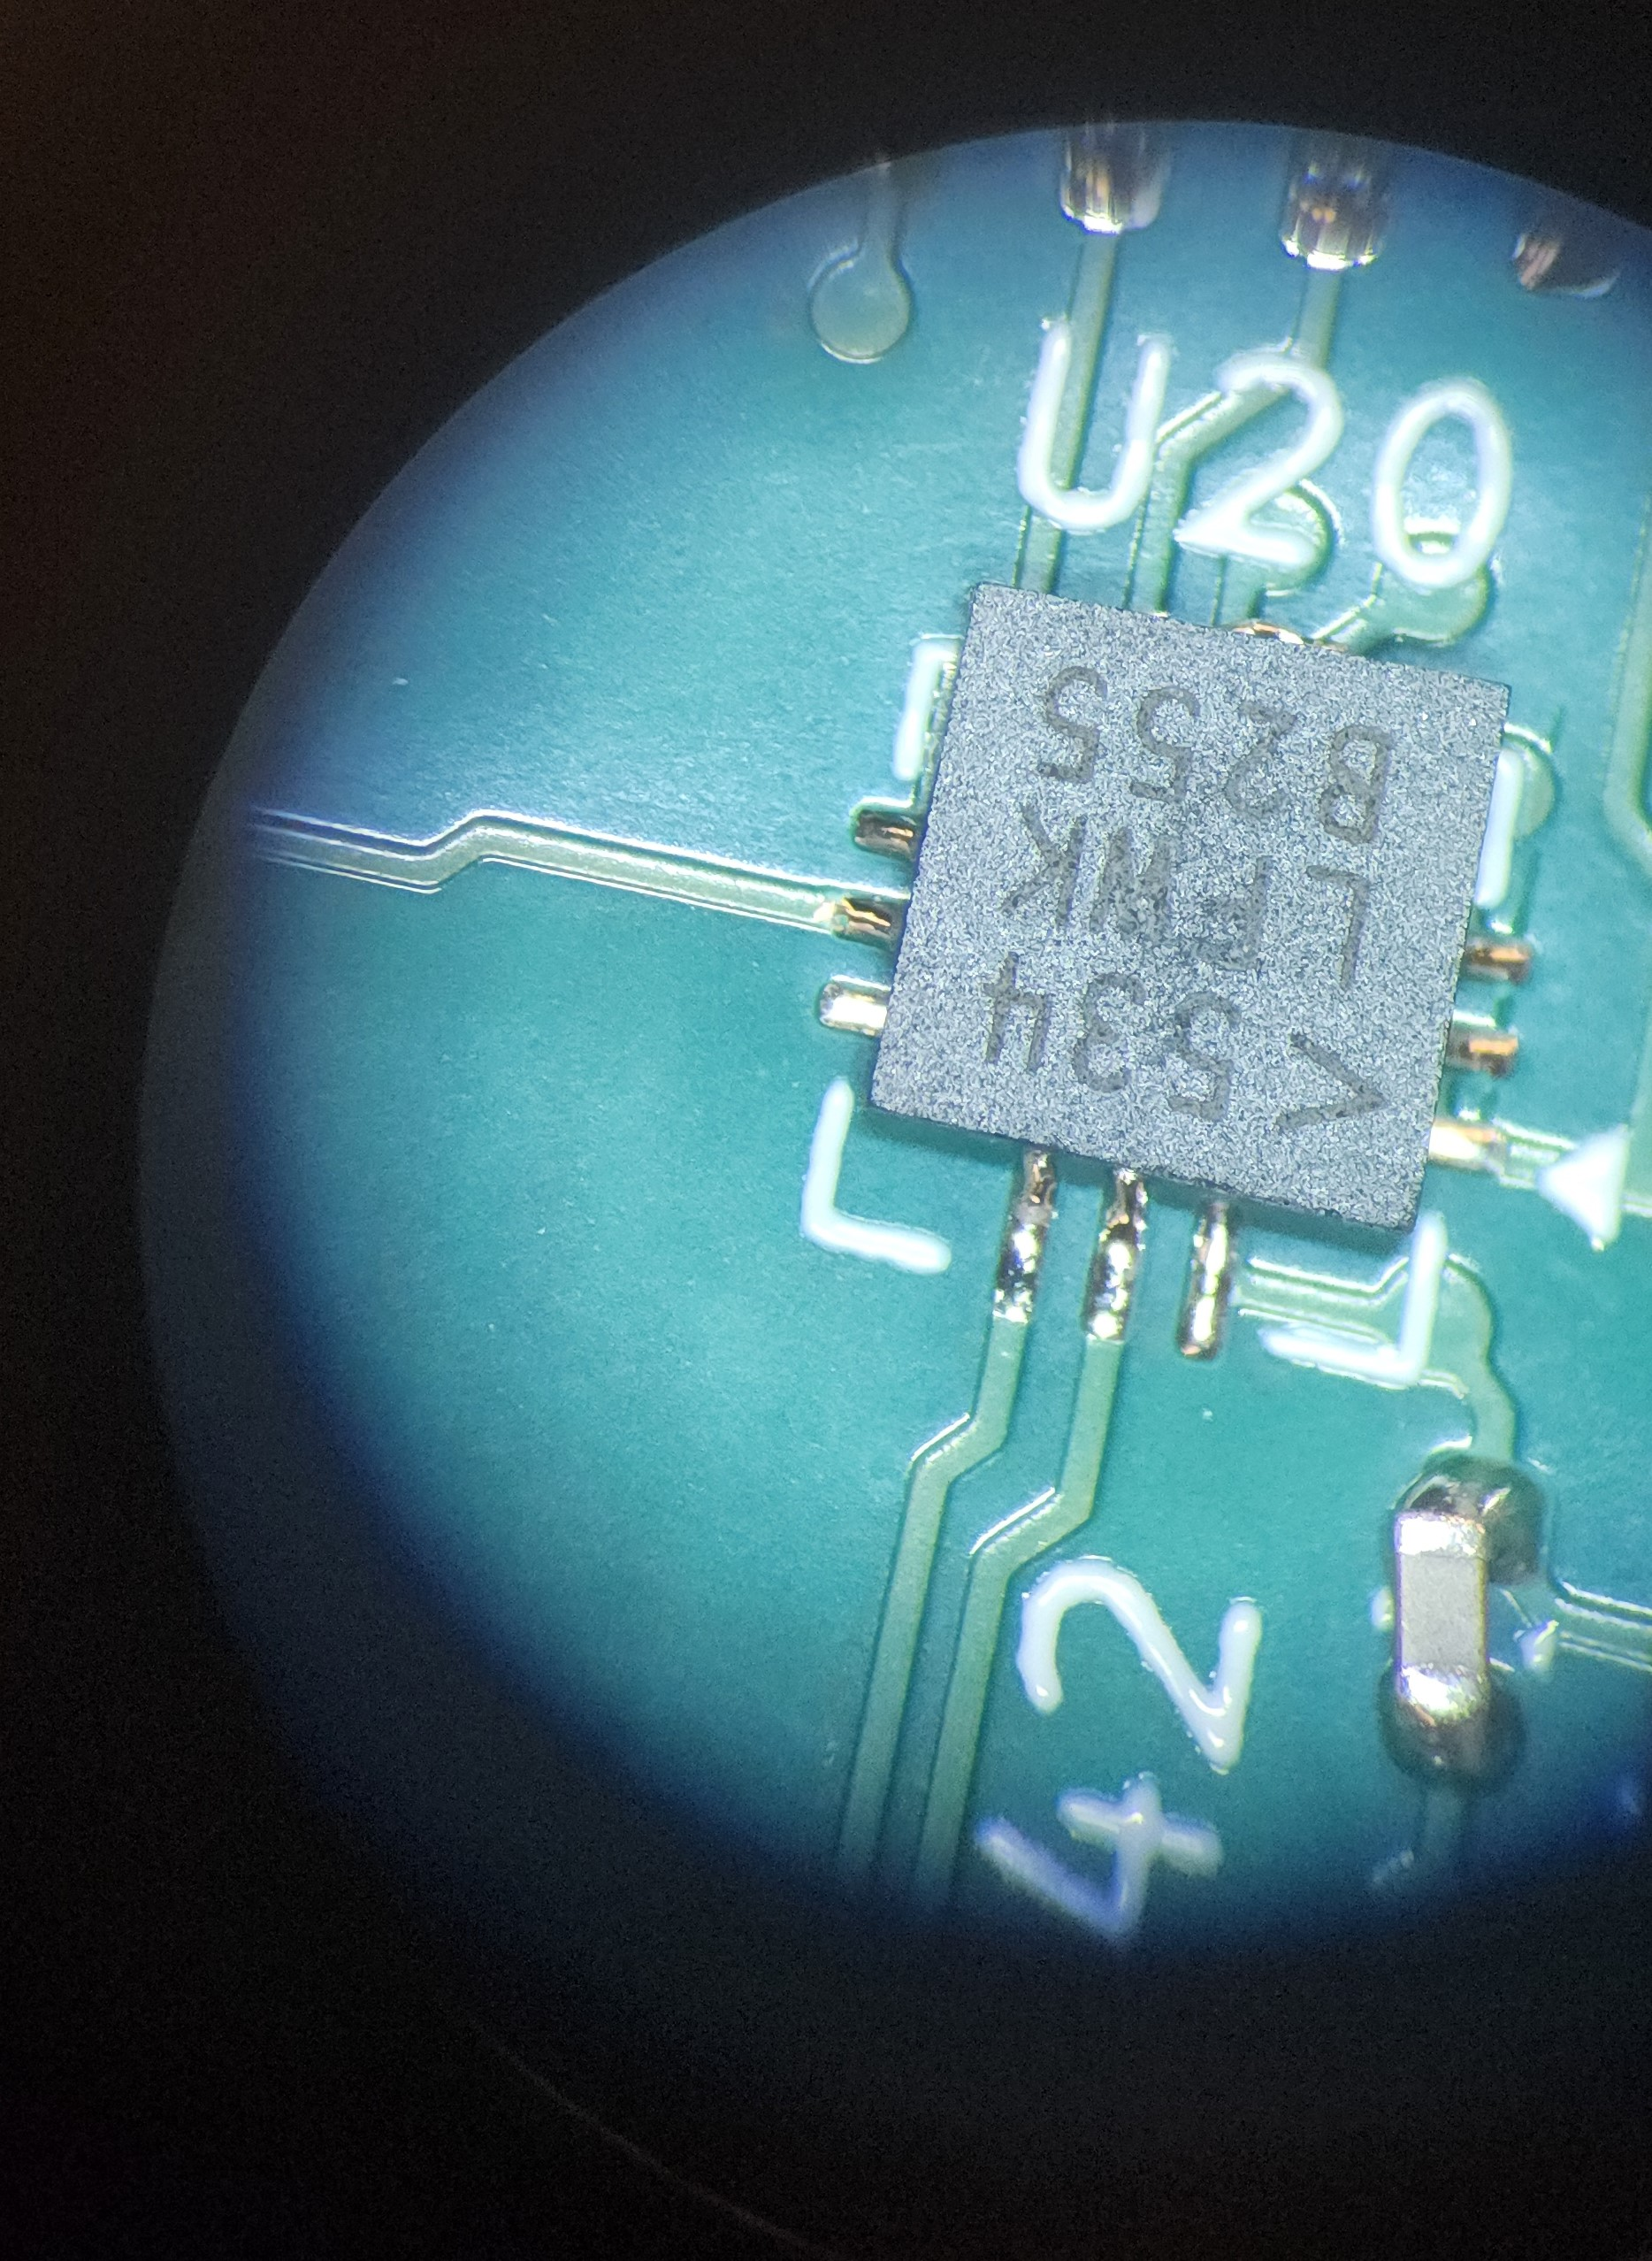
\includegraphics[
	width=3in,
	%height=0.85\textwidth,
	keepaspectratio
	]{Pictures/U20-Rework.jpg}
	\caption{The PMIC, U20, was found to have not been properly aligned when soldered initially, requiring rework to re-center the component.}
\end{figure}

\subsection{Smoke Test}
An open and short test was performed on the input and output side of the 'Sensor' board's regulator. Both the input and output side showed a charging capacitive load on the DMM (increasing resistance), and so it was deemed safe to proceed to power on testing.

A +5V supply was connected to the input, set for a 100mA current limit, and the board came up to approximately 3.6V. The current limit was increased to 500mA, and the bench supply came up to 5V and regulated. The output of the on-board regulator was verified to be putting out 3.3V. The microcontroller was observed to boot properly.


\section{I\texorpdfstring{$^2$}{2}C SDA Communication Problem}
\label{sec:i2c-sda-bringup}

\subsection{Initial Symptoms}

One of the first significant problems encountered during board bring-up was a failure
of the isolated I\textsuperscript{2}C interface. The Arduino firmware attempted to
communicate with the monitoring devices, but the expected responses were not received.
Because I\textsuperscript{2}C communication requires both the Serial Clock (SCL) and
Serial Data (SDA) signals to operate correctly, the two signals were examined at
multiple locations on the PCB using an oscilloscope.

During the initial measurements, unusual waveform shapes were observed on portions
of the isolated interface. These measurements were initially misleading because the
oscilloscope reference and the isolated circuit grounds were not connected as
intended. As I was taking measurements, working only on the +6VA supply initially to focus testing, I was measuring on both isolated and non-isolated side of the bus, and I was using floating bench supplies. After connecting all the supply commons, the waveforms were reasonable.

The SCL signal was then observed switching as expected, demonstrating that the
Arduino was attempting to generate I\textsuperscript{2}C transactions. The SDA path,
however, did not behave correctly. At one point in the signal chain the clock activity
was clearly visible, while the corresponding SDA-side output remained at a nearly
constant logic level. This indicated that the failure was not caused by the Arduino
failing to initiate communication, but was instead located within the SDA interface
circuitry.

With the sensor board disconnected, I was able to observe clock and data transmissions, with NACK visible on the 9th clock as below:
\begin{figure}[H]
	\centering
	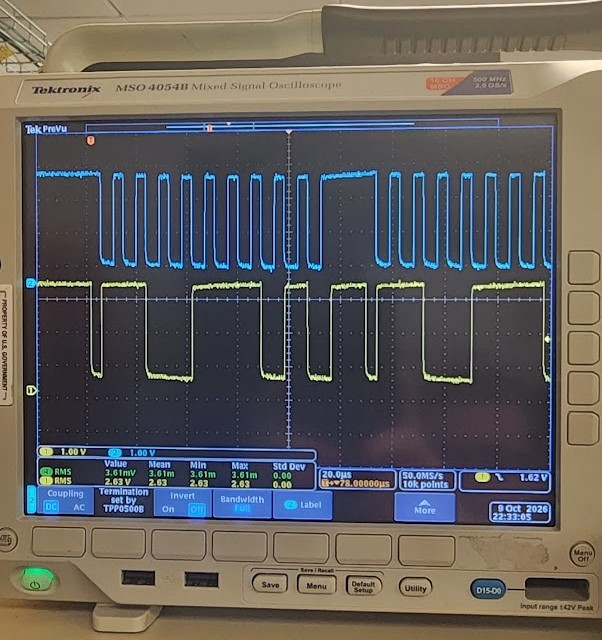
\includegraphics[
	width=3in,
	%height=0.85\textwidth,
	keepaspectratio
	]{Pictures/I2C_Sensor_Disconnected.jpg}
	\caption{I2C messages on Arduino shield cable driver output, with sensor board disconnected, NACK bit on 9th clock pulse}
\end{figure}


\subsection{SDA Signal Troubleshooting}

Troubleshooting proceeded by following the SDA signal through the circuit one node
at a time. The signal was measured on both sides of the isolation circuitry and at
the input and output of the associated logic circuitry. This approach made it possible
to determine where the expected transitions stopped propagating.

Testing showed that the input side of the isolation circuit was responding to SDA
activity. The voltage measured across the input device during a low state was
approximately \SI{1.34}{\volt}, indicating that the input element was being driven.
However, the corresponding output did not reproduce a valid SDA waveform.

Additional testing was performed with the pull-up and drive circuitry connected and
disconnected. The current limiting resistor for the optoisolators was dropped from 2k2\SI{}{\ohm} to \SI{909}{\ohm} resistor to ensure the drive current wasn't marginal, and the observed nodes only fell to approximately \SI{1.8}{\volt} during what should have
been a logic-low condition. This level was too high to provide a reliable digital
low for the following logic stage. It was behaving almost as if two push-pull outputs were fighting each other...

\subsection{Identification of Incorrect Component}
At this stage, I focused my attention around the PMIC's $\overline{SDAO}$ signal...Measuring the input pin of the optocoupler, I observed the line was being held high! This was expected behavior for I2C, except the selected part was designed to have an inverted SDA output!

Review of the schematic, assembled board, and component ordering information revealed
that the part populated in the SDA interface was not the intended device configuration.
Although the installed part was electrically similar to the device considered during
the design, its logic behavior did not match the requirements of the implemented
circuit.

I had ordered from Digikey the LTC2945IUD....the part required was the \textbf{LTC2945IUD-1}.

As a result, the output signal had the wrong logical relationship to the SDA signal
required by the remainder of the interface. The PCB therefore could not be corrected
through firmware alone. The hardware signal needed to be inverted before being
applied to the following stage.

This problem was not immediately obvious during assembly because the component was
physically compatible with the PCB footprint.

\subsection{Inverter Bodge Modification}

To continue board development without waiting on a parts order, a hardware
bodge was implemented to correct the SDA signal polarity. A Texas Instruments\\ SN74LVC2G04DCKR dual inverter was used for the modification, as an inverter I had on hand in the shop that was 3.3V compatible. The device contains two
independent logic inverters and operates from single supply voltage range compatible with
the logic used on the board. The DCK package is an SC-70-6 which is easily installed to the board with epoxy and tied into the circuit with 32awg magnet wire.

For the inverter channel used in the modification, pin~1 is the logic input and
pin~6 is the corresponding inverted output. The affected SDA-related signal was
therefore rerouted through this inverter before being connected to the following
stage. The modification provided the additional inversion required to produce the
logic polarity originally expected by the circuit.

The modification can be represented conceptually as

\begin{equation}
	V_{\mathrm{OUT}} = \overline{V_{\mathrm{IN}}},
\end{equation}

where \(V_{\mathrm{IN}}\) is the signal produced by the existing interface
and \(V_{\mathrm{OUT}}\) is the corrected signal applied to the following FET.

The bodge required cutting or and lifting the trace between the iso and the fet's gate, and adding short jumper wires between the existing circuit, the inverter input, and the fet gate. Power and ground were also provided to the inverter by tying into the optoisolator's 3.3V digital supply (via it's Pin 8, and the ground via pin 4).

\begin{figure}[H]
	\centering
	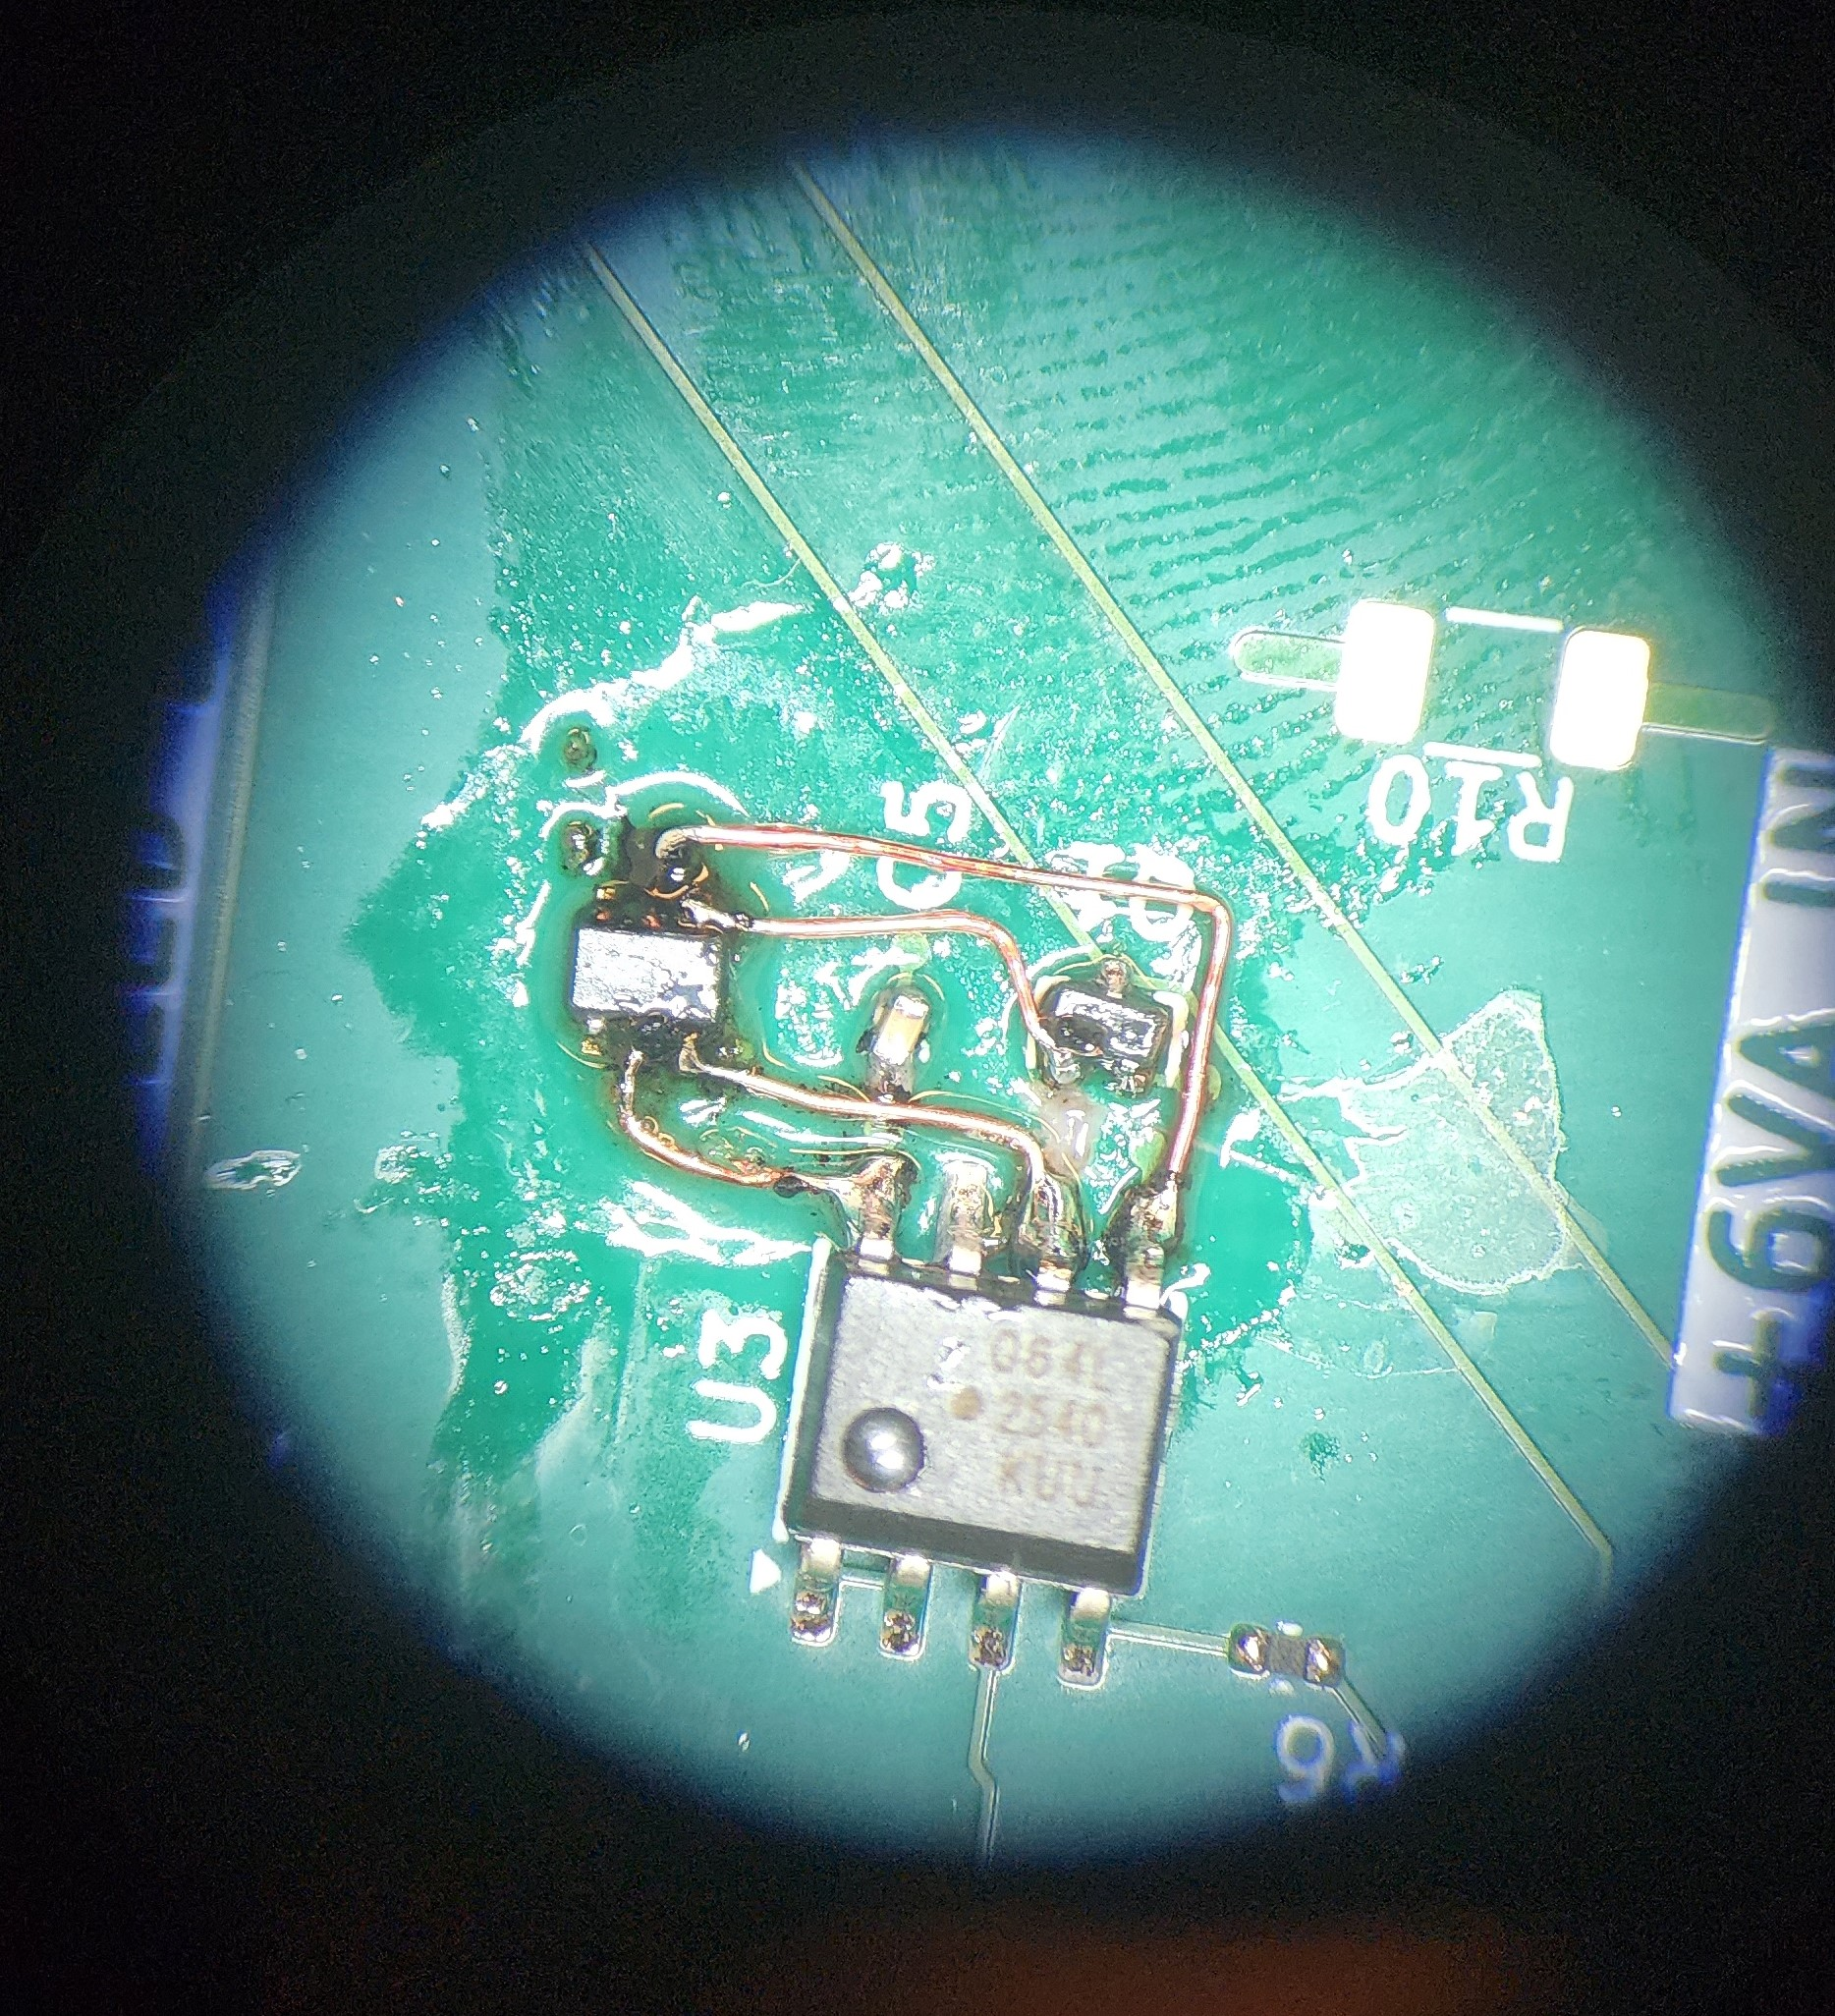
\includegraphics[
	width=4in,
	%height=0.85\textwidth,
	keepaspectratio
	]{Pictures/I2C-Inverter-Bodge.jpg}
	\caption{SC70-6 package inverter epoxied to the board, and 32awg bodge wires added, with cut trace, between optocoupler output and FET gate}
\end{figure}

\subsection{Verification After Modification}
After implementing the SDA modification, the SDA signal was inspected
once again using an oscilloscope at several points in the communication circuit.
The reason for this inspection was not only to check the presence of a waveform,
but also to see whether there was proper propagation of logic-high and
logic-low signals through the entire interface.

This signal was checked alongside the SCL waveform during the I\textsuperscript{2}C
communication by the Arduino. The focus of observation was on the ninth clock pulse,
which is where an I\textsuperscript{2}C slave should acknowledge the transmission
by lowering the SDA signal. This observation was important since it showed that the
process was moving further than before modification.

After confirming the waveforms, once again, communication was tested through the
firmware. Success in communication after modification proved that the error
occurred at the hardware stage of the SDA signal implementation and not within
the I\textsuperscript{2}C software itself.

\begin{figure}[H]
	\centering
	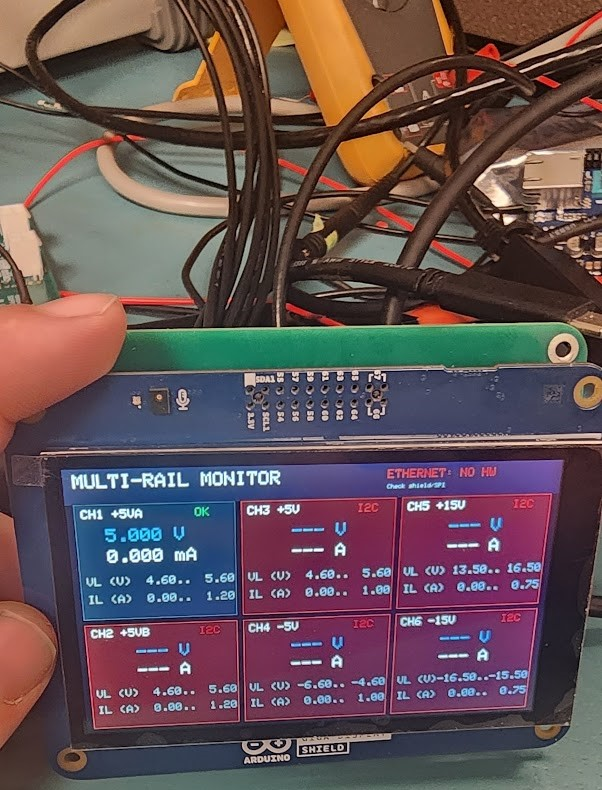
\includegraphics[
	width=3in,
	%height=0.85\textwidth,
	keepaspectratio
	]{Pictures/5V_PMIC_I2C_Fixed.jpg}
	\caption{Communication is now working for the +5VA channel that has had the I2C connection repaired. The other 5 channels have had the FET gate floated (copper traces cut and lifted) from the opto to release the data bus, but have not yet had their inverters installed.}
\end{figure}

The troubleshooting process used to locate the problem can be summarized as:

\begin{enumerate}
	\item Confirm that the required circuit power supplies are present.
	\item Establish the correct oscilloscope ground reference for each isolated
	portion of the circuit.
	\item Verify that the Arduino generates I\textsuperscript{2}C clock activity.
	\item Probe SDA sequentially through each stage of the interface.
	\item Identify the point where valid SDA transitions are lost.
	\item Compare the installed component and its logic behavior with the schematic
	requirements.
	\item Modify the circuit to correct the signal polarity.
	\item Re-measure the SDA waveform.
	\item Repeat the firmware communication test.
\end{enumerate}

The error was helpful in the bring-up of the board since it showed that
embedded system debugging must consider both the hardware and the software at the
same time. The error of the firmware showing communication problems via I\textsuperscript{2}C showed the symptom but using the oscilloscope to measure the values pointed out where the exact problem was located.

\subsection{Further Bodges and Repairs}
Repairs were carried out on the remaining 5 channels. Additionally, it was found that the +5VA and -5V both had the same I2C address configured; this was modified by removing U20, cutting the traces to the address pins, and running 30awg magnet wire to tie Pin 3 to INTVCC (via U21-8) and Pin 2 to -5V via C43-2. Power was restored and then it was observed to now be working on all 6 channels! 

\begin{figure}[H]
	\centering
	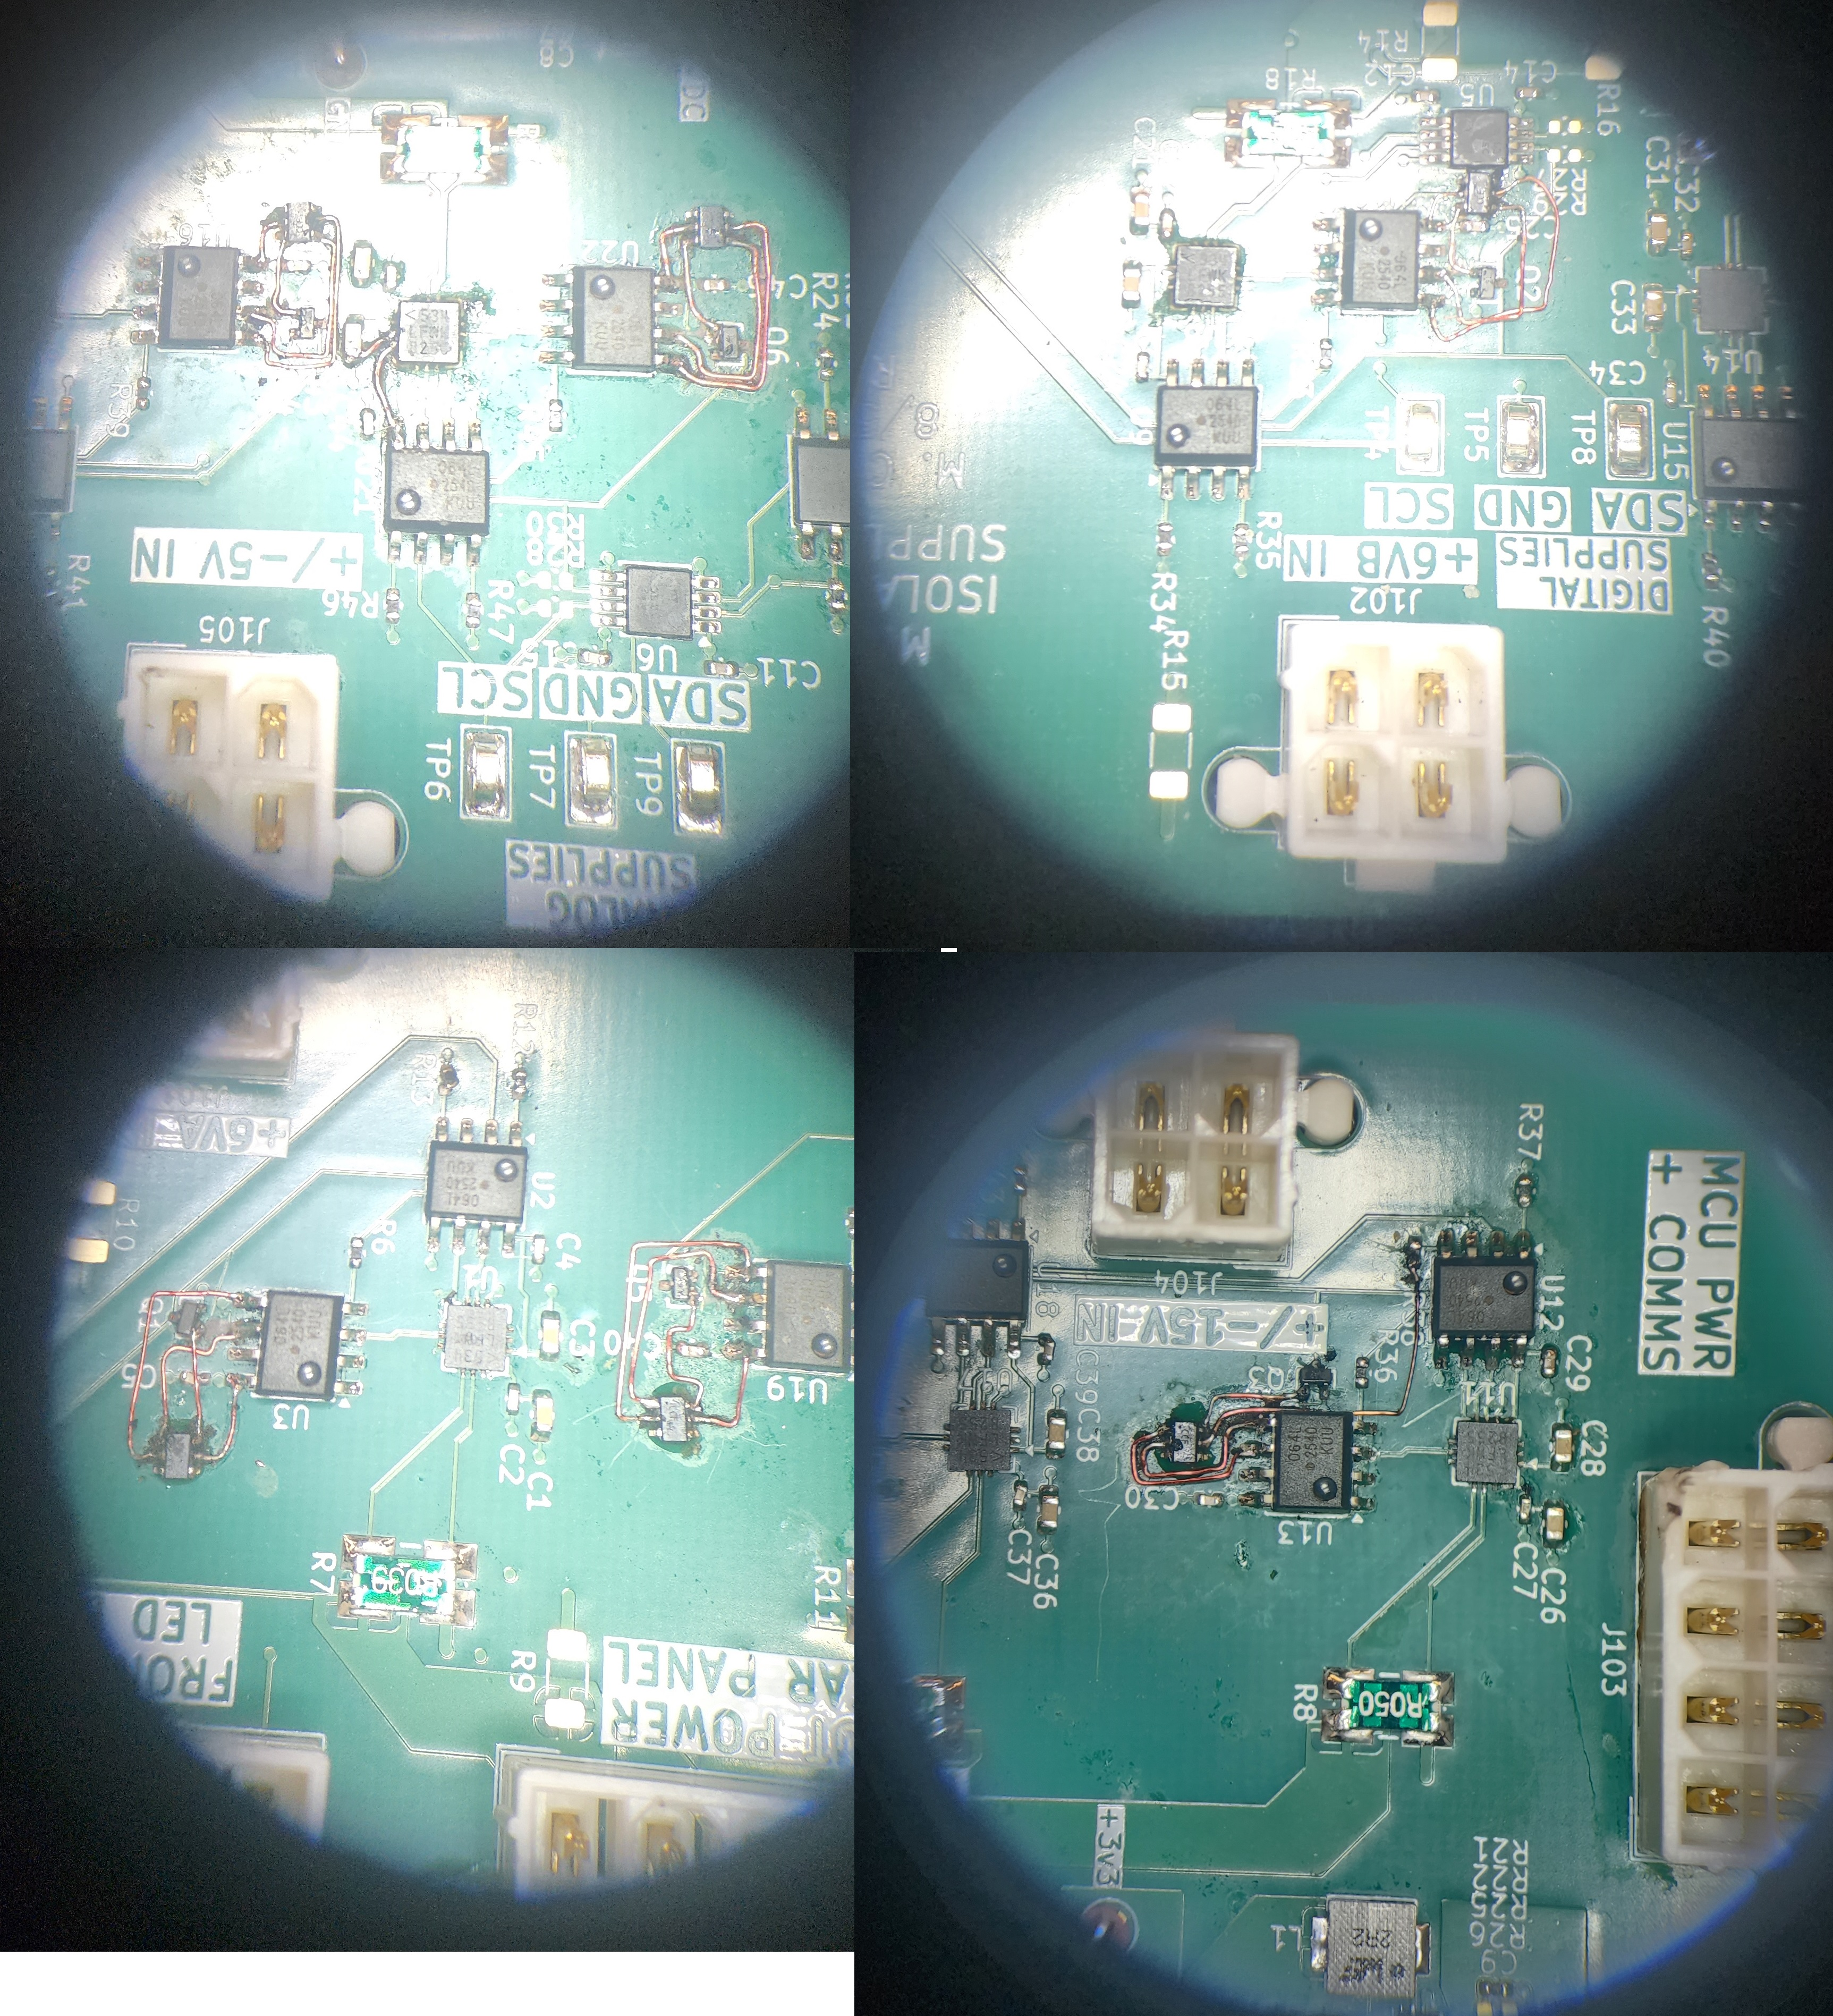
\includegraphics[
	width=\textwidth,
	%height=0.85\textwidth,
	keepaspectratio
	]{Pictures/AllChanRework.jpg}
	\caption{Rework is completed for all 6 channels}
\end{figure}

\begin{figure}[H]
	\centering
	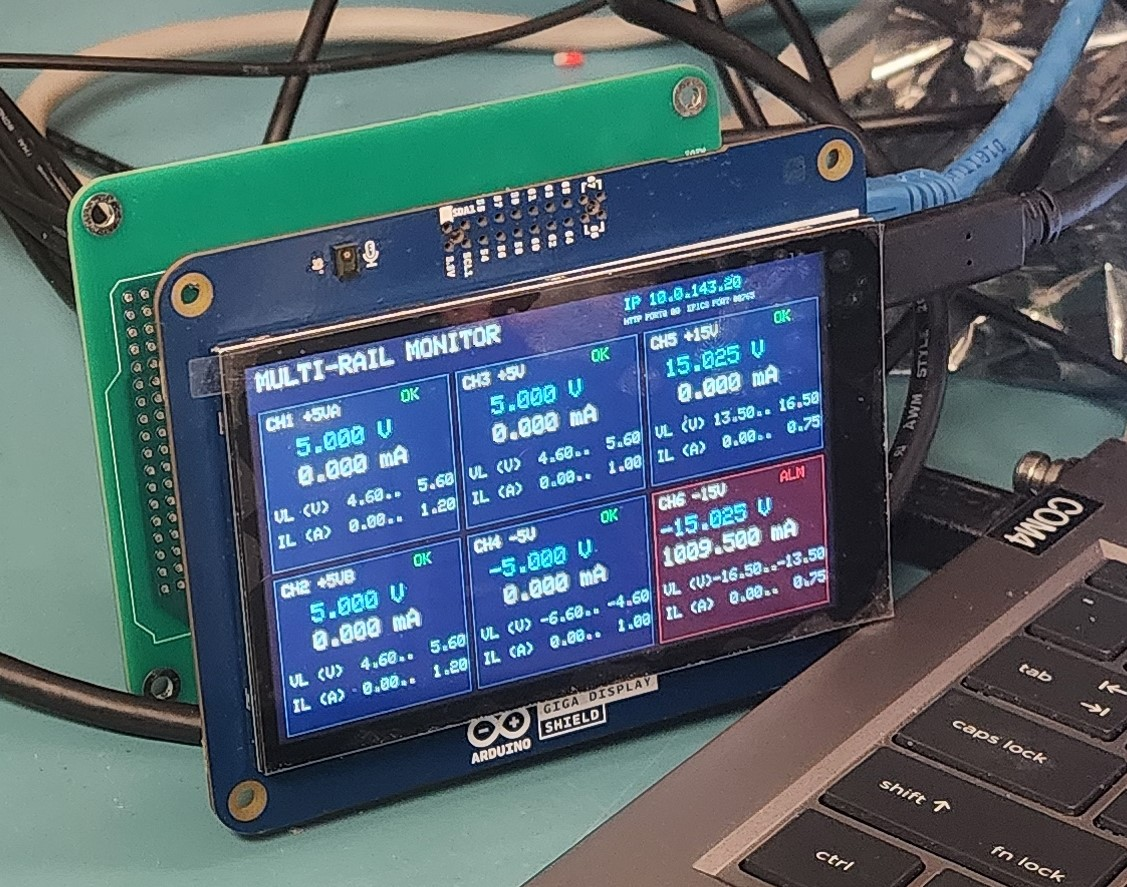
\includegraphics[
	width=\textwidth,
	%height=0.85\textwidth,
	keepaspectratio
	]{Pictures/TestAllCommsWorking.jpg}
	\caption{All 6 channels now working!}
\end{figure}

\begin{figure}[H]
	\centering
	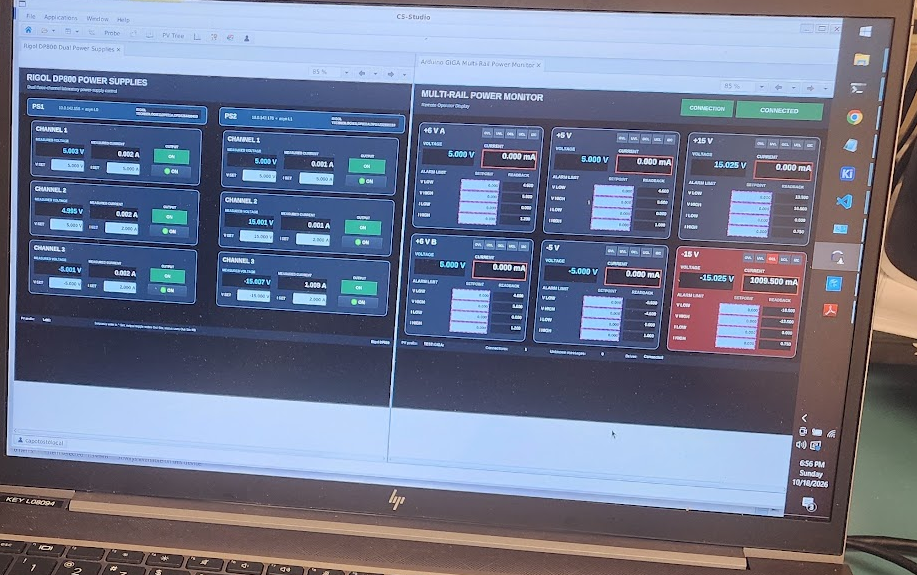
\includegraphics[
	width=\textwidth,
	%height=0.85\textwidth,
	keepaspectratio
	]{Pictures/CSSScreen.png}
	\caption{Control Panels working as well, showing 1A dummy load on one channel}
\end{figure}

